
\documentclass[paper=a4, fontsize=11pt]{scrartcl} % A4 paper and 11pt font size

\usepackage[T1]{fontenc} % Use 8-bit encoding that has 256 glyphs
\usepackage{fourier} % Use the Adobe Utopia font for the document - comment this line to return to the LaTeX default
\usepackage[english]{babel} % English language/hyphenation
\usepackage{amsmath,amsfonts,amsthm} % Math packages

\usepackage{lipsum} % Used for inserting dummy 'Lorem ipsum' text into the template
\usepackage{tikz}
\usepackage{amsmath}
\usepackage{sectsty} % Allows customizing section commands
\allsectionsfont{\centering \normalfont\scshape} % Make all sections centered, the default font and small caps

\usepackage{fancyhdr} % Custom headers and footers
\pagestyle{fancyplain} % Makes all pages in the document conform to the custom headers and footers
\fancyhead{} % No page header - if you want one, create it in the same way as the footers below
\fancyfoot[L]{} % Empty left footer
\fancyfoot[C]{} % Empty center footer
\fancyfoot[R]{\thepage} % Page numbering for right footer
\renewcommand{\headrulewidth}{0pt} % Remove header underlines
\renewcommand{\footrulewidth}{0pt} % Remove footer underlines
\setlength{\headheight}{13.6pt} % Customize the height of the header
\usepackage{float}
\numberwithin{equation}{section} % Number equations within sections (i.e. 1.1, 1.2, 2.1, 2.2 instead of 1, 2, 3, 4)
\numberwithin{figure}{section} % Number figures within sections (i.e. 1.1, 1.2, 2.1, 2.2 instead of 1, 2, 3, 4)
\numberwithin{table}{section} % Number tables within sections (i.e. 1.1, 1.2, 2.1, 2.2 instead of 1, 2, 3, 4)

\setlength\parindent{0pt} % Removes all indentation from paragraphs - comment this line for an assignment with lots of text

%----------------------------------------------------------------------------------------
%	TITLE SECTION
%----------------------------------------------------------------------------------------

\newcommand{\horrule}[1]{\rule{\linewidth}{#1}} % Create horizontal rule command with 1 argument of height

\title{	
\normalfont \normalsize 
\textsc{California State University San Marcos \\ Dr. De Leone, Physics 323} \\ [25pt] % Your university, school and/or department name(s)
\horrule{0.5pt} \\[0.4cm] % Thin top horizontal rule
\huge H.W. 2\\ % The assignment title
\horrule{2pt} \\[0.5cm] % Thick bottom horizontal rule
}

\author{Josh Lucas} % Your name

\date{\normalsize\today} % Today's date or a custom date

\begin{document}

\maketitle % Print the title

%----------------------------------------------------------------------------------------
%	PROBLEM 1
%----------------------------------------------------------------------------------------

\section{Electron Spin and Magnetic Moment}
Two spheres are spinning with the same angular momentum, but oriented differently. Which sphere experiences the larger force from the magnetic field? 


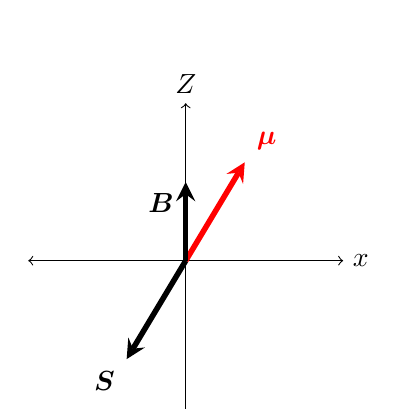
\begin{tikzpicture}
 % \draw[thin,gray!40] (-2,-2) grid (2,2);
  \draw[<->] (-2,0)--(2,0) node[right]{$x$};
  \draw[<->] (0,-2)--(0,2) node[above]{$Z$};
  \draw[line width=2pt,red,-stealth](0,0)--(0.75,1.25) node[anchor=south west]{$\boldsymbol{\mu}$};
  \draw[line width=2pt,black,-stealth](0,0)--(-0.75,-1.25) node[anchor=north east]{$\boldsymbol{S}$};
   \draw[line width=2pt,black,-stealth](0,0)--(0,1) node[anchor=north east]{$\boldsymbol{B}$};
\end{tikzpicture}
(A)
\hspace{45mm}
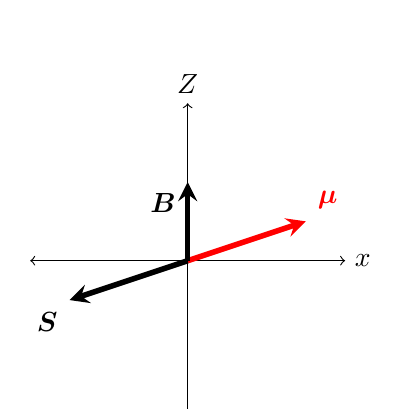
\begin{tikzpicture}
  %\draw[thin,gray!40] (-2,-2) grid (2,2);
  \draw[<->] (-2,0)--(2,0) node[right]{$x$};
  \draw[<->] (0,-2)--(0,2) node[above]{$Z$};
  \draw[line width=2pt,red,-stealth](0,0)--(1.5,.5) node[anchor=south west]{$\boldsymbol{\mu}$};
  \draw[line width=2pt,black,-stealth](0,0)--(-1.5,-.5) node[anchor=north east]{$\boldsymbol{S}$};
 \draw[line width=2pt,black,-stealth](0,0)--(0,1) node[anchor=north east]{$\boldsymbol{B}$};
\end{tikzpicture}
(B)

The magnitude of the Z component of the magnetic moment, $\vec{\mu}$ of the electron will determine the force on the atom in the homogeneous magnetic field, $\vec{B}$, \textbf{in a classical system}. As the Z component grows so does the force experienced on the electron until it is parallel with the field. The direction of the electron's magnetic moment's poles, with the direction of $\vec{\mu}$ being north, compared to the magnetic field's poles will determine the direction of the force. When the components are orthogonal the force is zero. 
\begin{equation*}
F_z \approx -g\frac{e}{2me}S_z\frac{\partial B_z}{\partial Z}
\end{equation*}
Because the magnetic field is decreasing there can be a net force on the electron in one direction or another. 

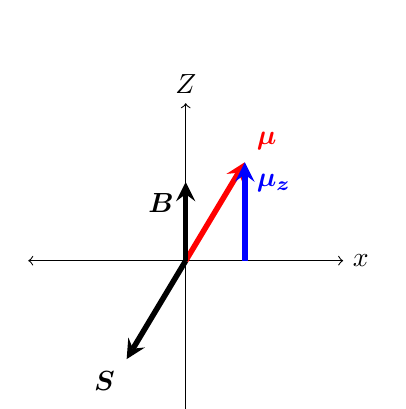
\begin{tikzpicture}
 % \draw[thin,gray!40] (-2,-2) grid (2,2);
  \draw[<->] (-2,0)--(2,0) node[right]{$x$};
  \draw[<->] (0,-2)--(0,2) node[above]{$Z$};
  \draw[line width=2pt,red,-stealth](0,0)--(0.75,1.25) node[anchor=south west]{$\boldsymbol{\mu}$};
  \draw[line width=2pt,black,-stealth](0,0)--(-0.75,-1.25) node[anchor=north east]{$\boldsymbol{S}$};
   \draw[line width=2pt,black,-stealth](0,0)--(0,1) node[anchor=north east]{$\boldsymbol{B}$};
    \draw[line width=2pt,blue,-stealth](0.75,0)--(0.75,1.25) node[anchor=north west]{$\boldsymbol{\mu_z}$};
\end{tikzpicture}
(A)
\hspace{45mm}
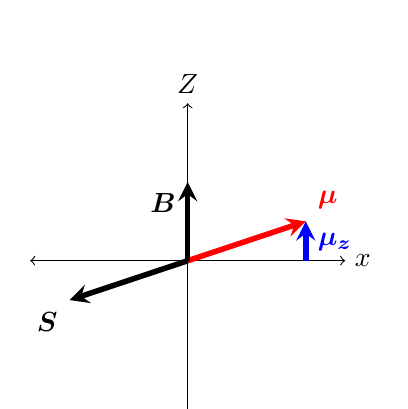
\begin{tikzpicture}
 % \draw[thin,gray!40] (-2,-2) grid (2,2);
  \draw[<->] (-2,0)--(2,0) node[right]{$x$};
  \draw[<->] (0,-2)--(0,2) node[above]{$Z$};
   \draw[line width=2pt,red,-stealth](0,0)--(1.5,.5) node[anchor=south west]{$\boldsymbol{\mu}$};
  \draw[line width=2pt,black,-stealth](0,0)--(-1.5,-.5) node[anchor=north east]{$\boldsymbol{S}$};
   \draw[line width=2pt,black,-stealth](0,0)--(0,1) node[anchor=north east]{$\boldsymbol{B}$};
    \draw[line width=2pt,blue,-stealth](1.5,0)--(1.5,.5) node[anchor=north west]{$\boldsymbol{\mu_z}$};
\end{tikzpicture}
(B)
\newline
\\
We can also use the relation of $ \vec{\mu} \cdot \vec{B} = |\vec{\mu}||\vec{B}| \cos{\theta} $, where theta is the angle between the magnetic moment and the direction of the $\vec{B}$ field. If the angle is $\frac{\pi}{2}$, the force is zero. If the angle is over $\frac{\pi}{2}$, then the force changes direction. 
The figure \textbf{A's} magnetic moment has a \textbf{larger} Z component in the direction of the field creating a \textbf{larger force }on the particle according to classical speculations. 

%------------------------------------------------


%----------------------------------------------------------------------------------------

\end{document}